\documentclass{article}
\usepackage{graphicx}
\usepackage{subcaption}
\usepackage[margin=1.0in]{geometry}
\setlength\parindent{0pt}
\usepackage[titletoc]{appendix}


\begin{document}

\title{Live Coding Visualisation Study Report - DRAFT}
\author{Arrian Purcell}

\maketitle

\begin{figure}[t]
\centering
\begin{subfigure}{.5\textwidth}
    \centering
    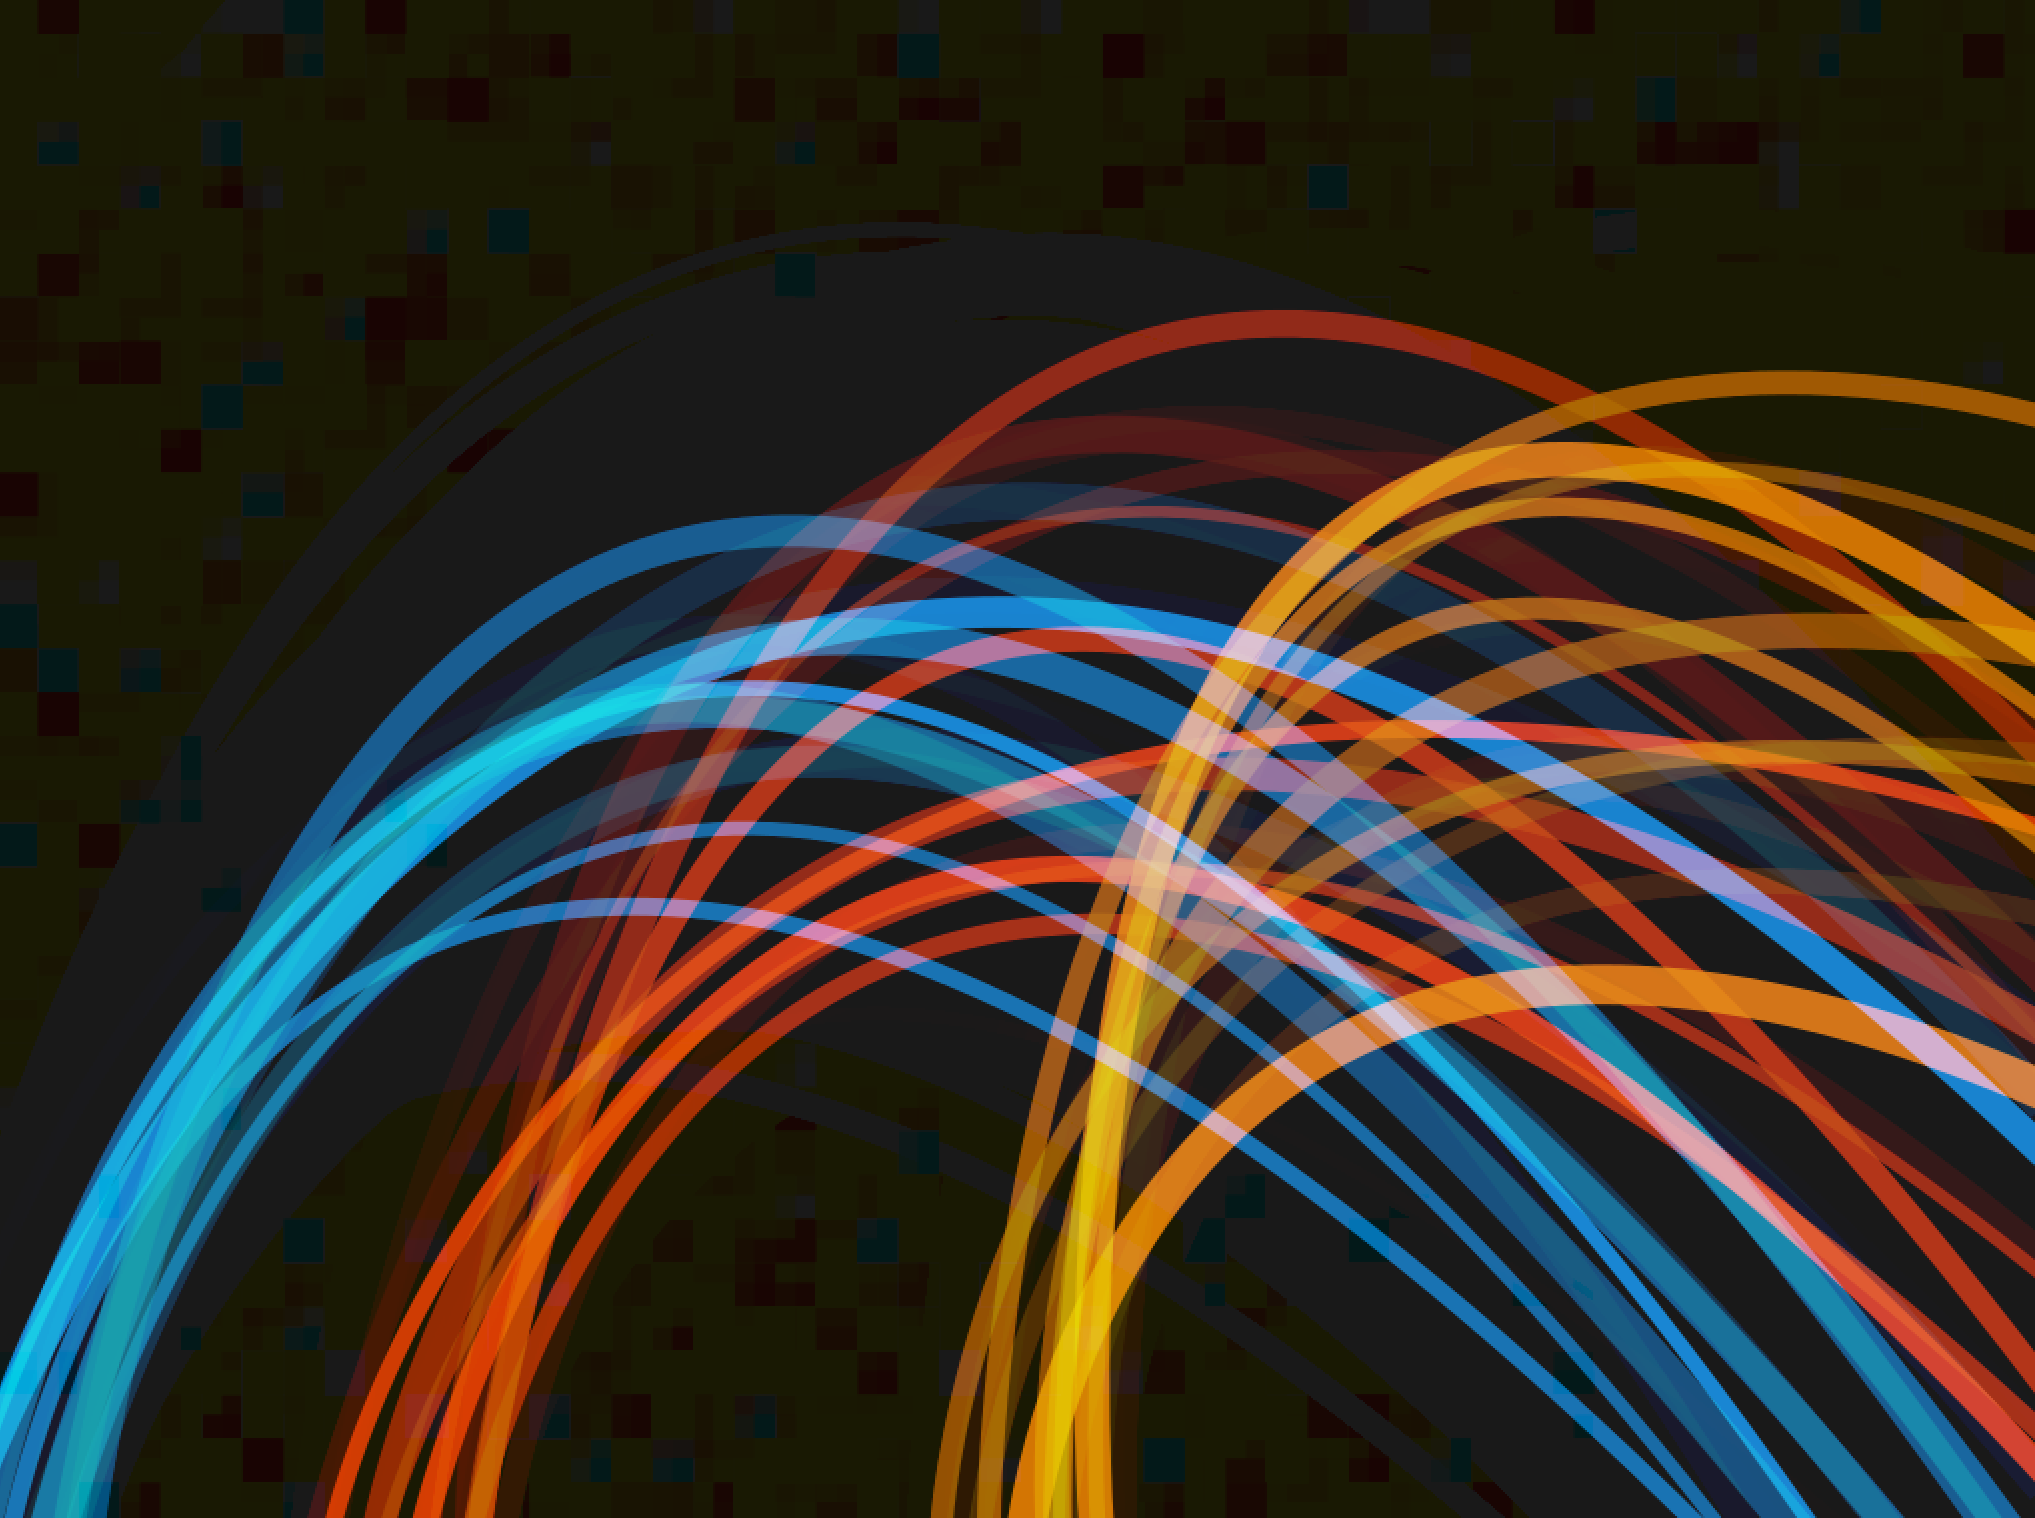
\includegraphics[width=0.9\linewidth]{aesthetic-vis.png}
    \caption{Aesthetic Visualisation}
    \label{avis}
\end{subfigure}%
\begin{subfigure}{.5\textwidth}
    \centering
    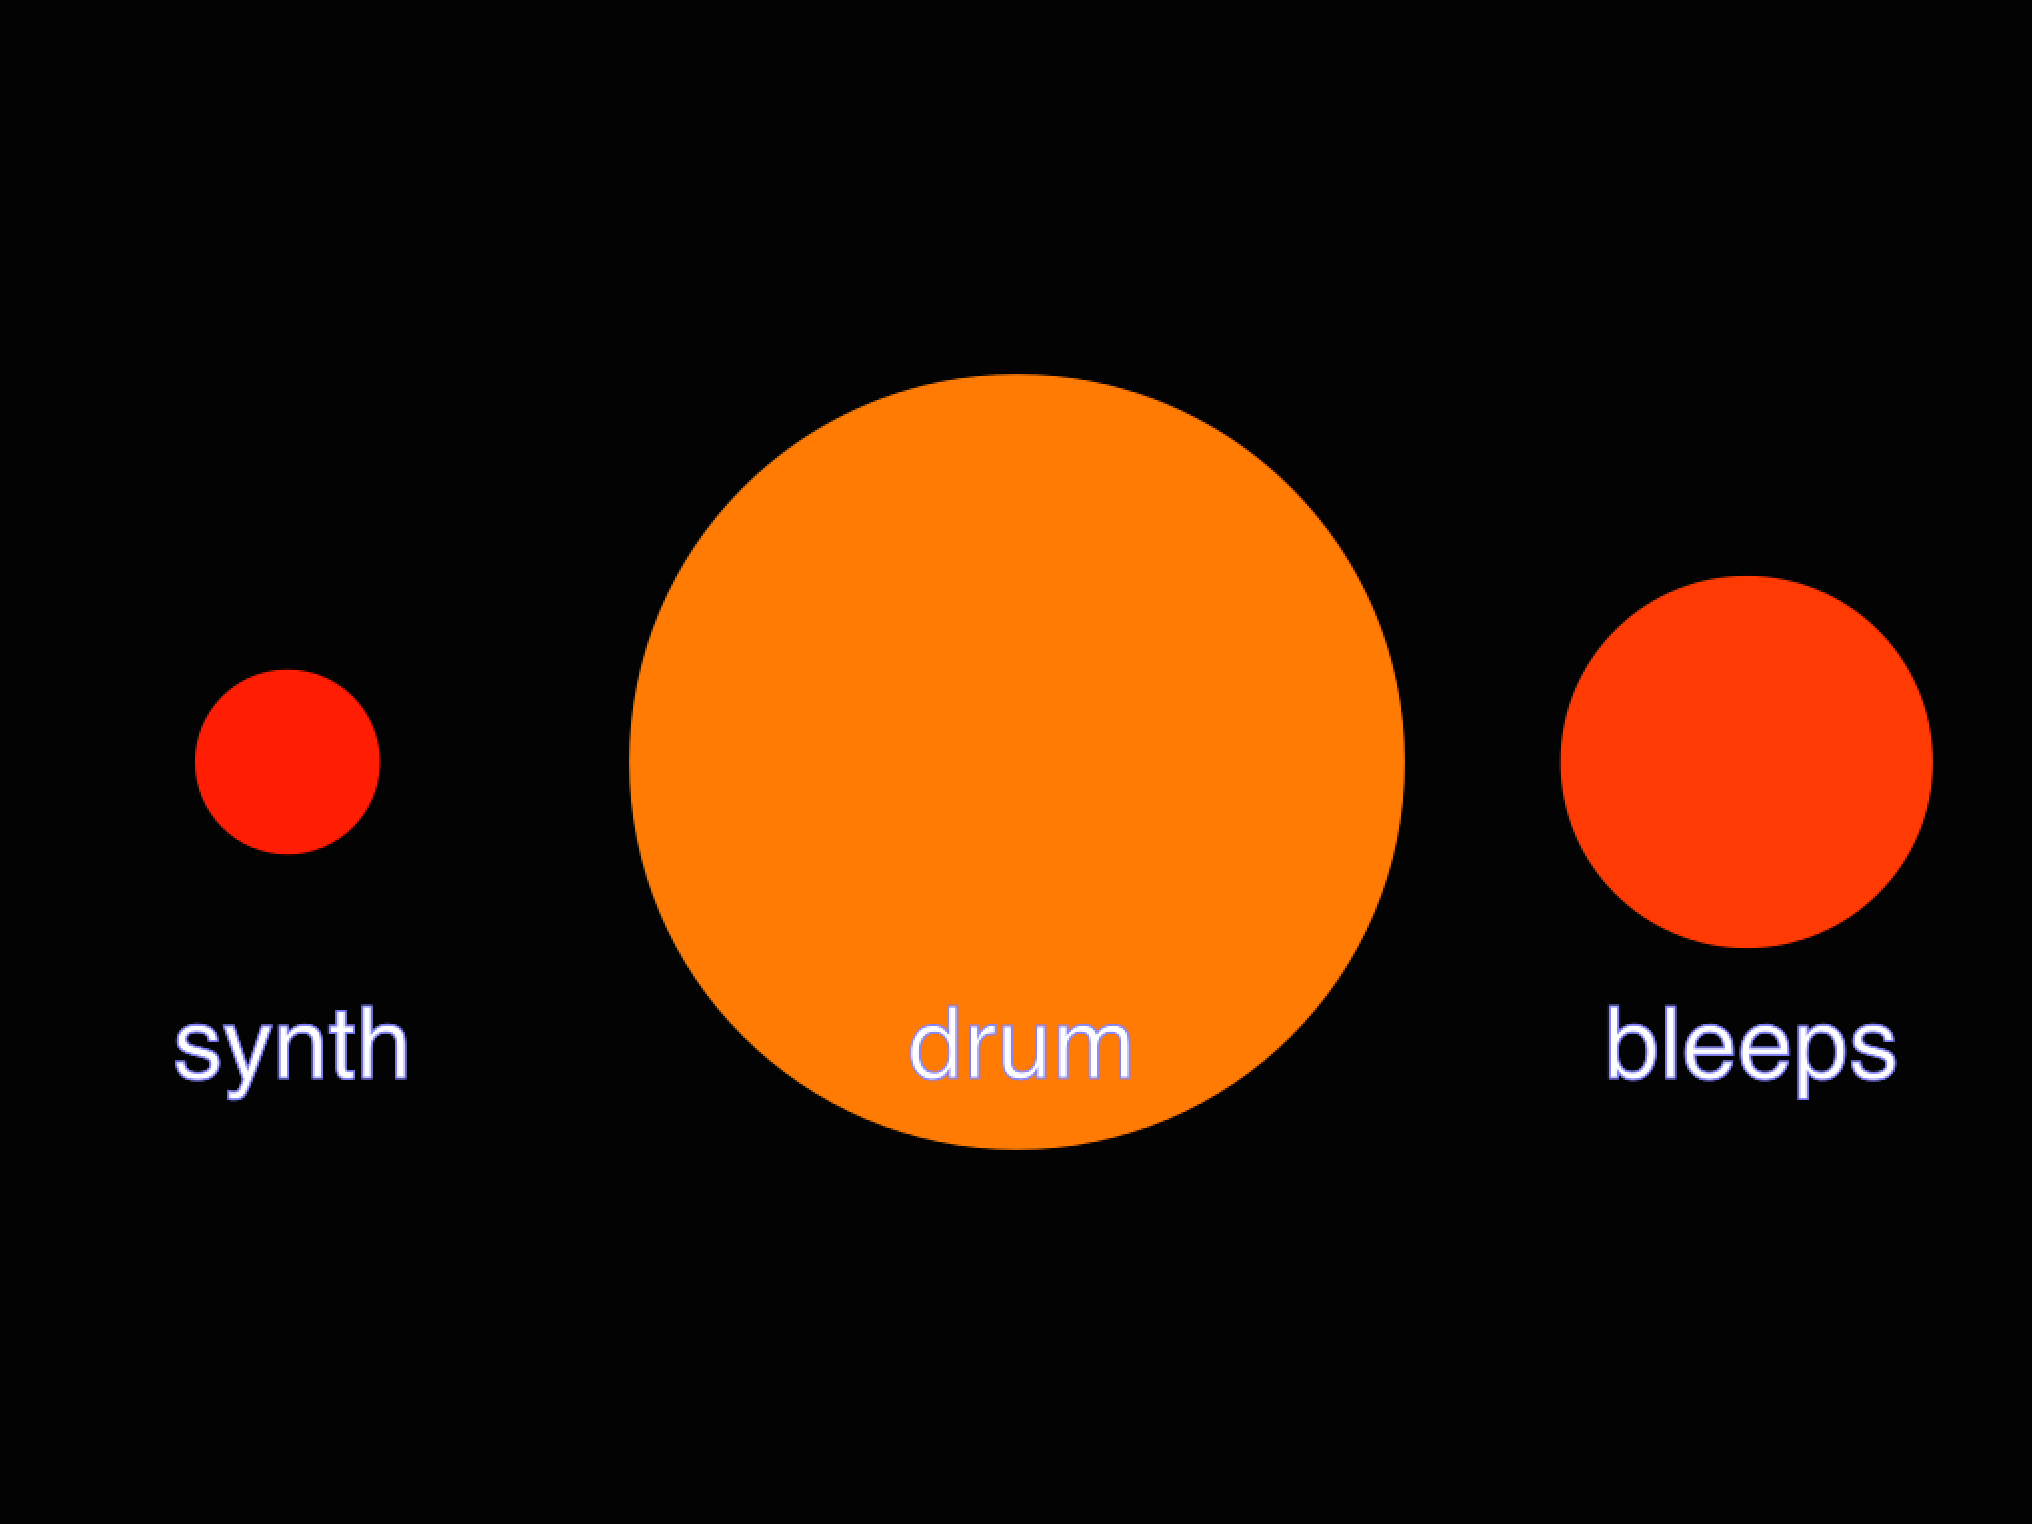
\includegraphics[width=0.9\linewidth]{didactic-vis.png}
    \caption{Didactic Visualisation}
    \label{dvis}
\end{subfigure}
\caption{Visualisation Examples}
\end{figure}


Two visualisations in the context of a live coding performance have been analysed to determine effective presentational and educational features. The two visualsations tested included a visualisation targetting aesthetic appeal and a visualisation with a more didactic approach. The goal was to determine differences between the two approaches in order to inform future live coding visualisations.\\

The didactic visusalisations predominantly focussed on the relationship to the programs functions, prominantly displaying the names of the active functions with visual indication of the number of functions running and their callback time. Bright colours and solid shapes were used to ensure the intention of the code was communicated. An example of this approach can be seen in Figure \ref{dvis}.\\

The aesthetic visualisation focussed less on the programmatic aspects of the performance, intending to provide additional visual interest to the projected code. To this end, more variety was used in visual structure and colour. An example of this approach can be seen in Figure \ref{avis}.


\section{Method}
Two live coding performances were conducted with separate participant groups. Each performance was divided into two sets of ten minutes demonstrating one of the two experimental visualisation conditions including the aesthetic condition and the didactic condition. The order in which these two conditions were presented to the audience was swapped over the two performances.\\

After explaining to the parcipants the order and the high level intention of the experiment and allowing the participants to complete the initial demographic section of a survey, the live coder began a performance set utilising one type of visualisation with music. Following this first set, some survey questions were administered to the participants asking them specifically about their enjoyment and undertstanding related to the visualisations. A second set was then played using the alternative visualisation. Following this second set, the same survey questions were adminstered again, again asking the particiants specfics about their enjoyment and understanding related to the specific visualisation demonstrated. A final survey question was then asked relating to their opinion regarding the whole performance and suggested improvements.

\section{Participants}

A total of 41 participants took part in the study. $66\%$ of the participants stated that they were male (see Figure \ref{genderdistribution}) and most participants were aged between 18 and 32 ($76\%$, see Figure \ref{agedistribution}). As the study was conducted within the Computer Science Department, a large proportion of the participants were experienced with programming with $90\%$ having current or previous experience with it. Nevertheless, only $15\%$ of participants had previous experience with any of the Lisp style languages.\\

Of the participants, $68\%$ stated that they listened to a large amount of music (see Figure \ref{musicdistribution}) though only about $15\%$ of participants stated that they played and instrument or sung regularly (see Figure \ref{instrumentdistribution}). Only $22\%$ of participants had seen a live coding performance before.\\

Over the two performances, 19 participants observed the first performance and 22 participants observed the second performance. The demographic makeup of the two performances were very similar.

\begin{figure}[t]
\centering
\begin{subfigure}{.5\textwidth}
    \centering
    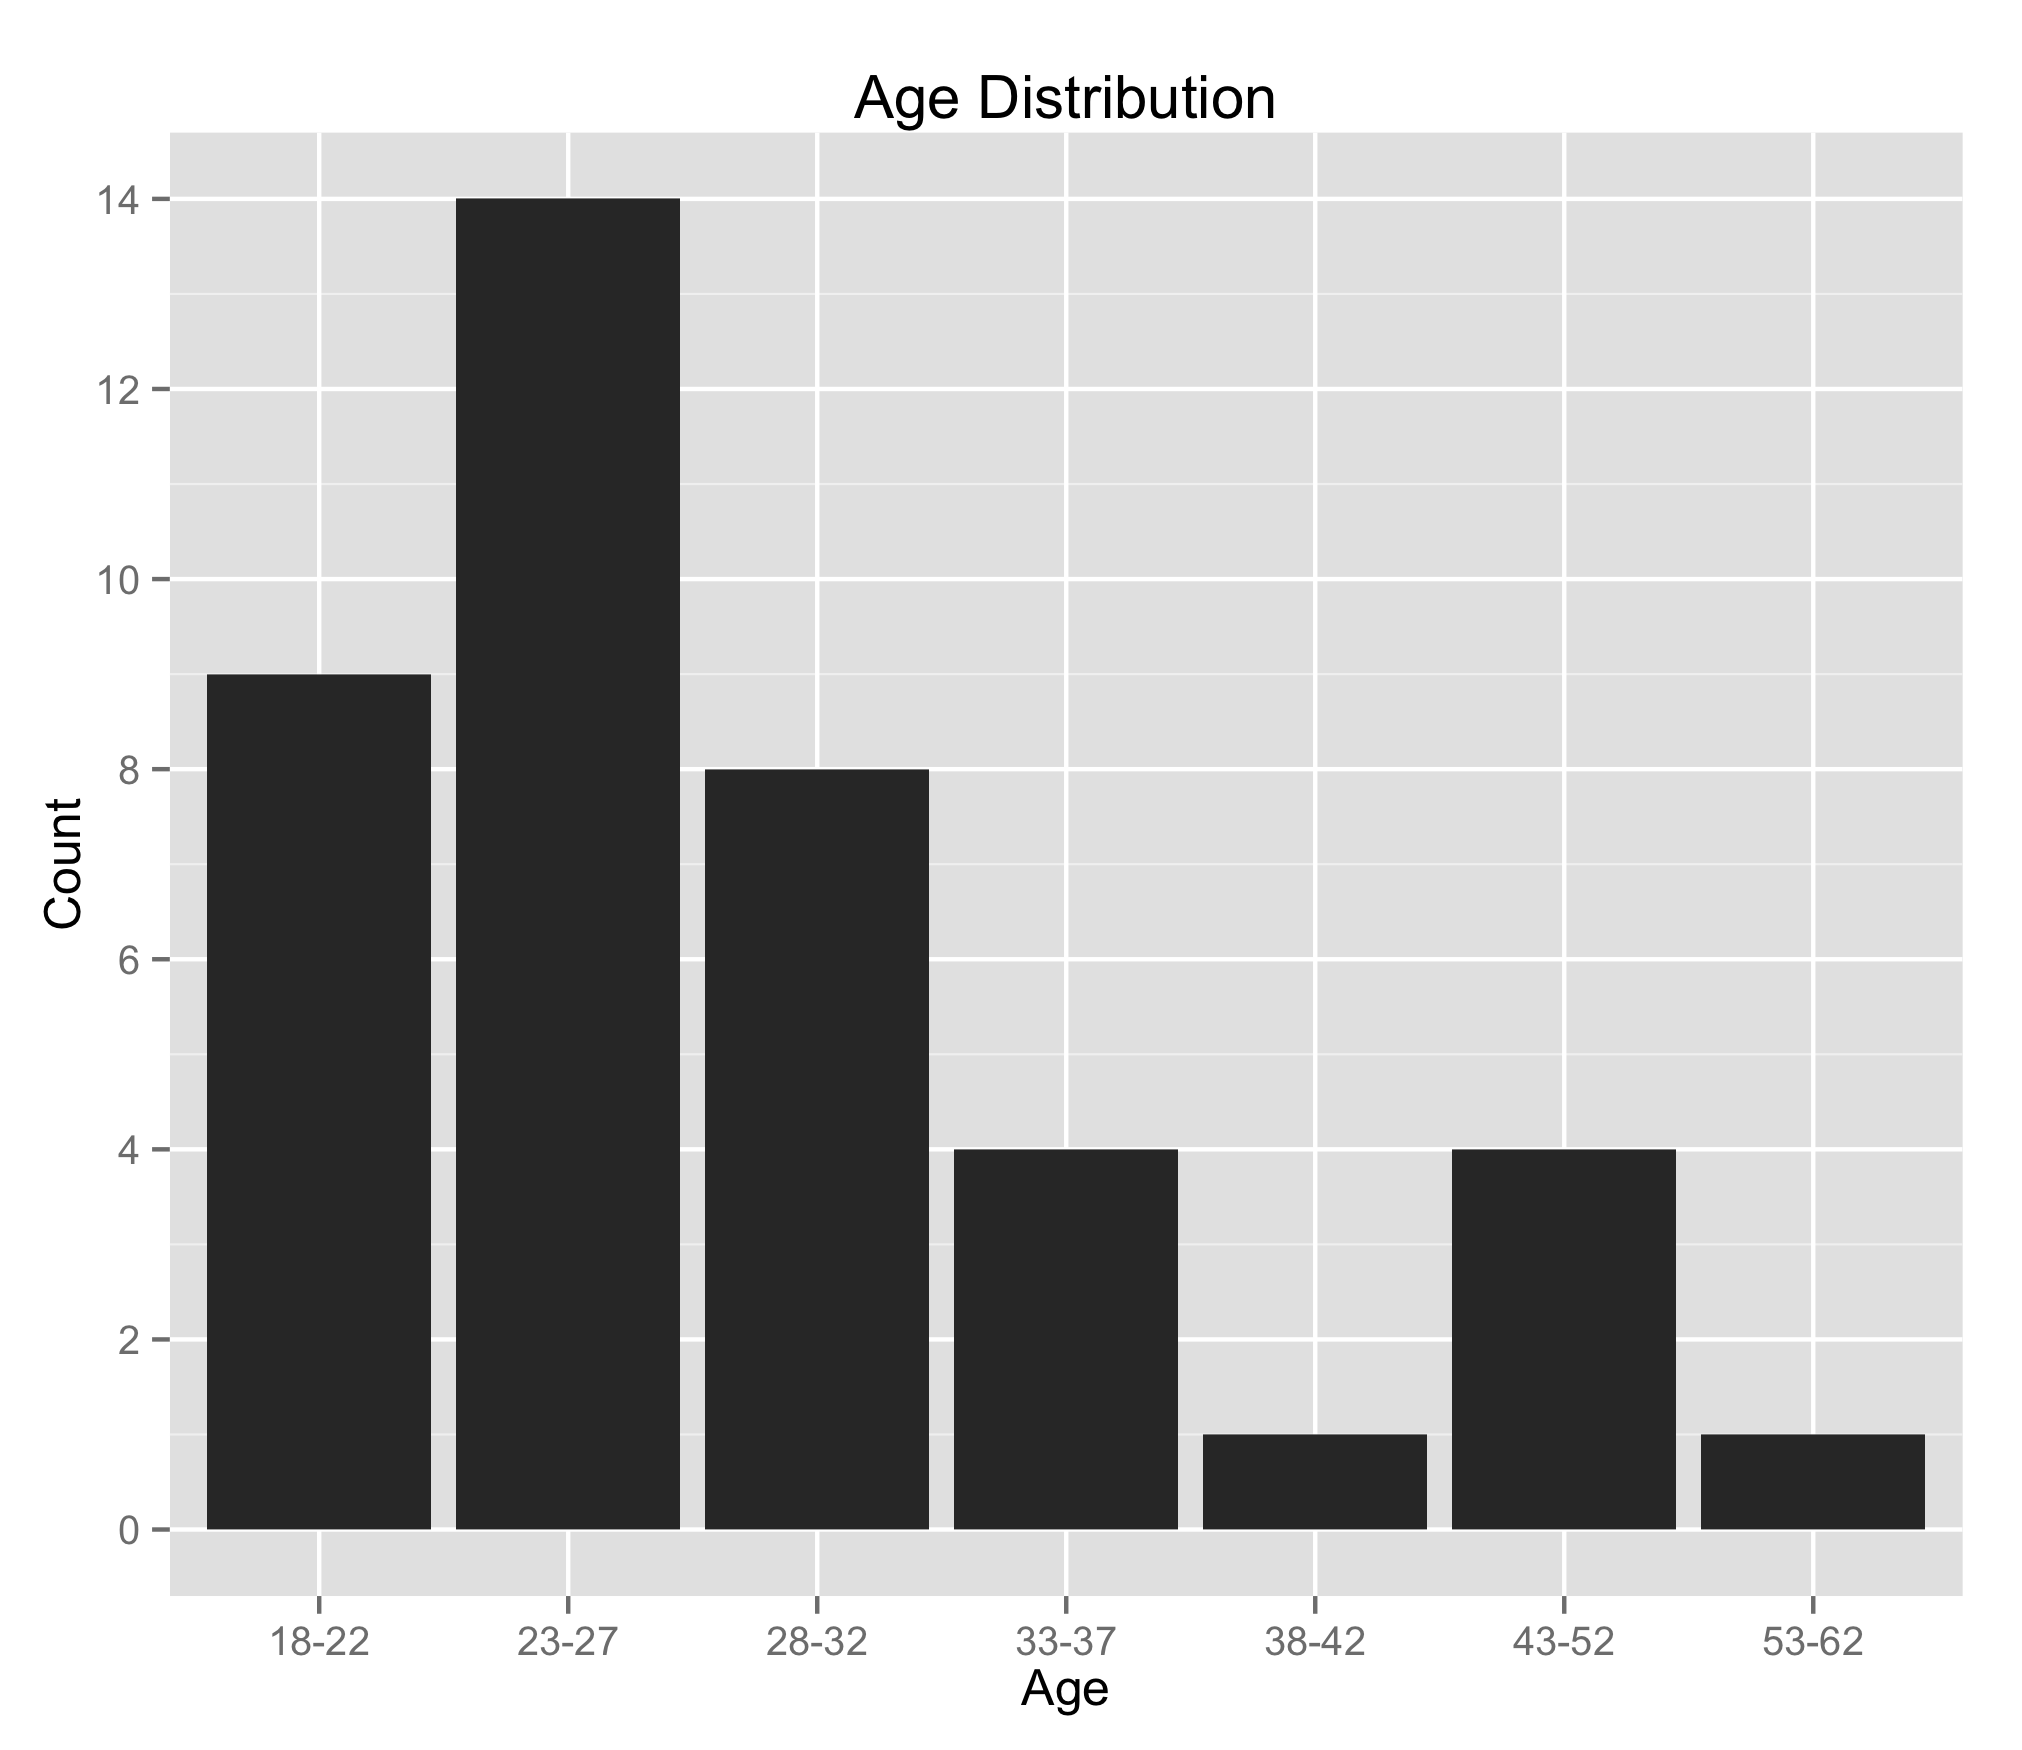
\includegraphics[width=1.0\linewidth]{age.png}
    \caption{Age Distribution}
    \label{agedistribution}
\end{subfigure}%
\begin{subfigure}{.5\textwidth}
    \centering
    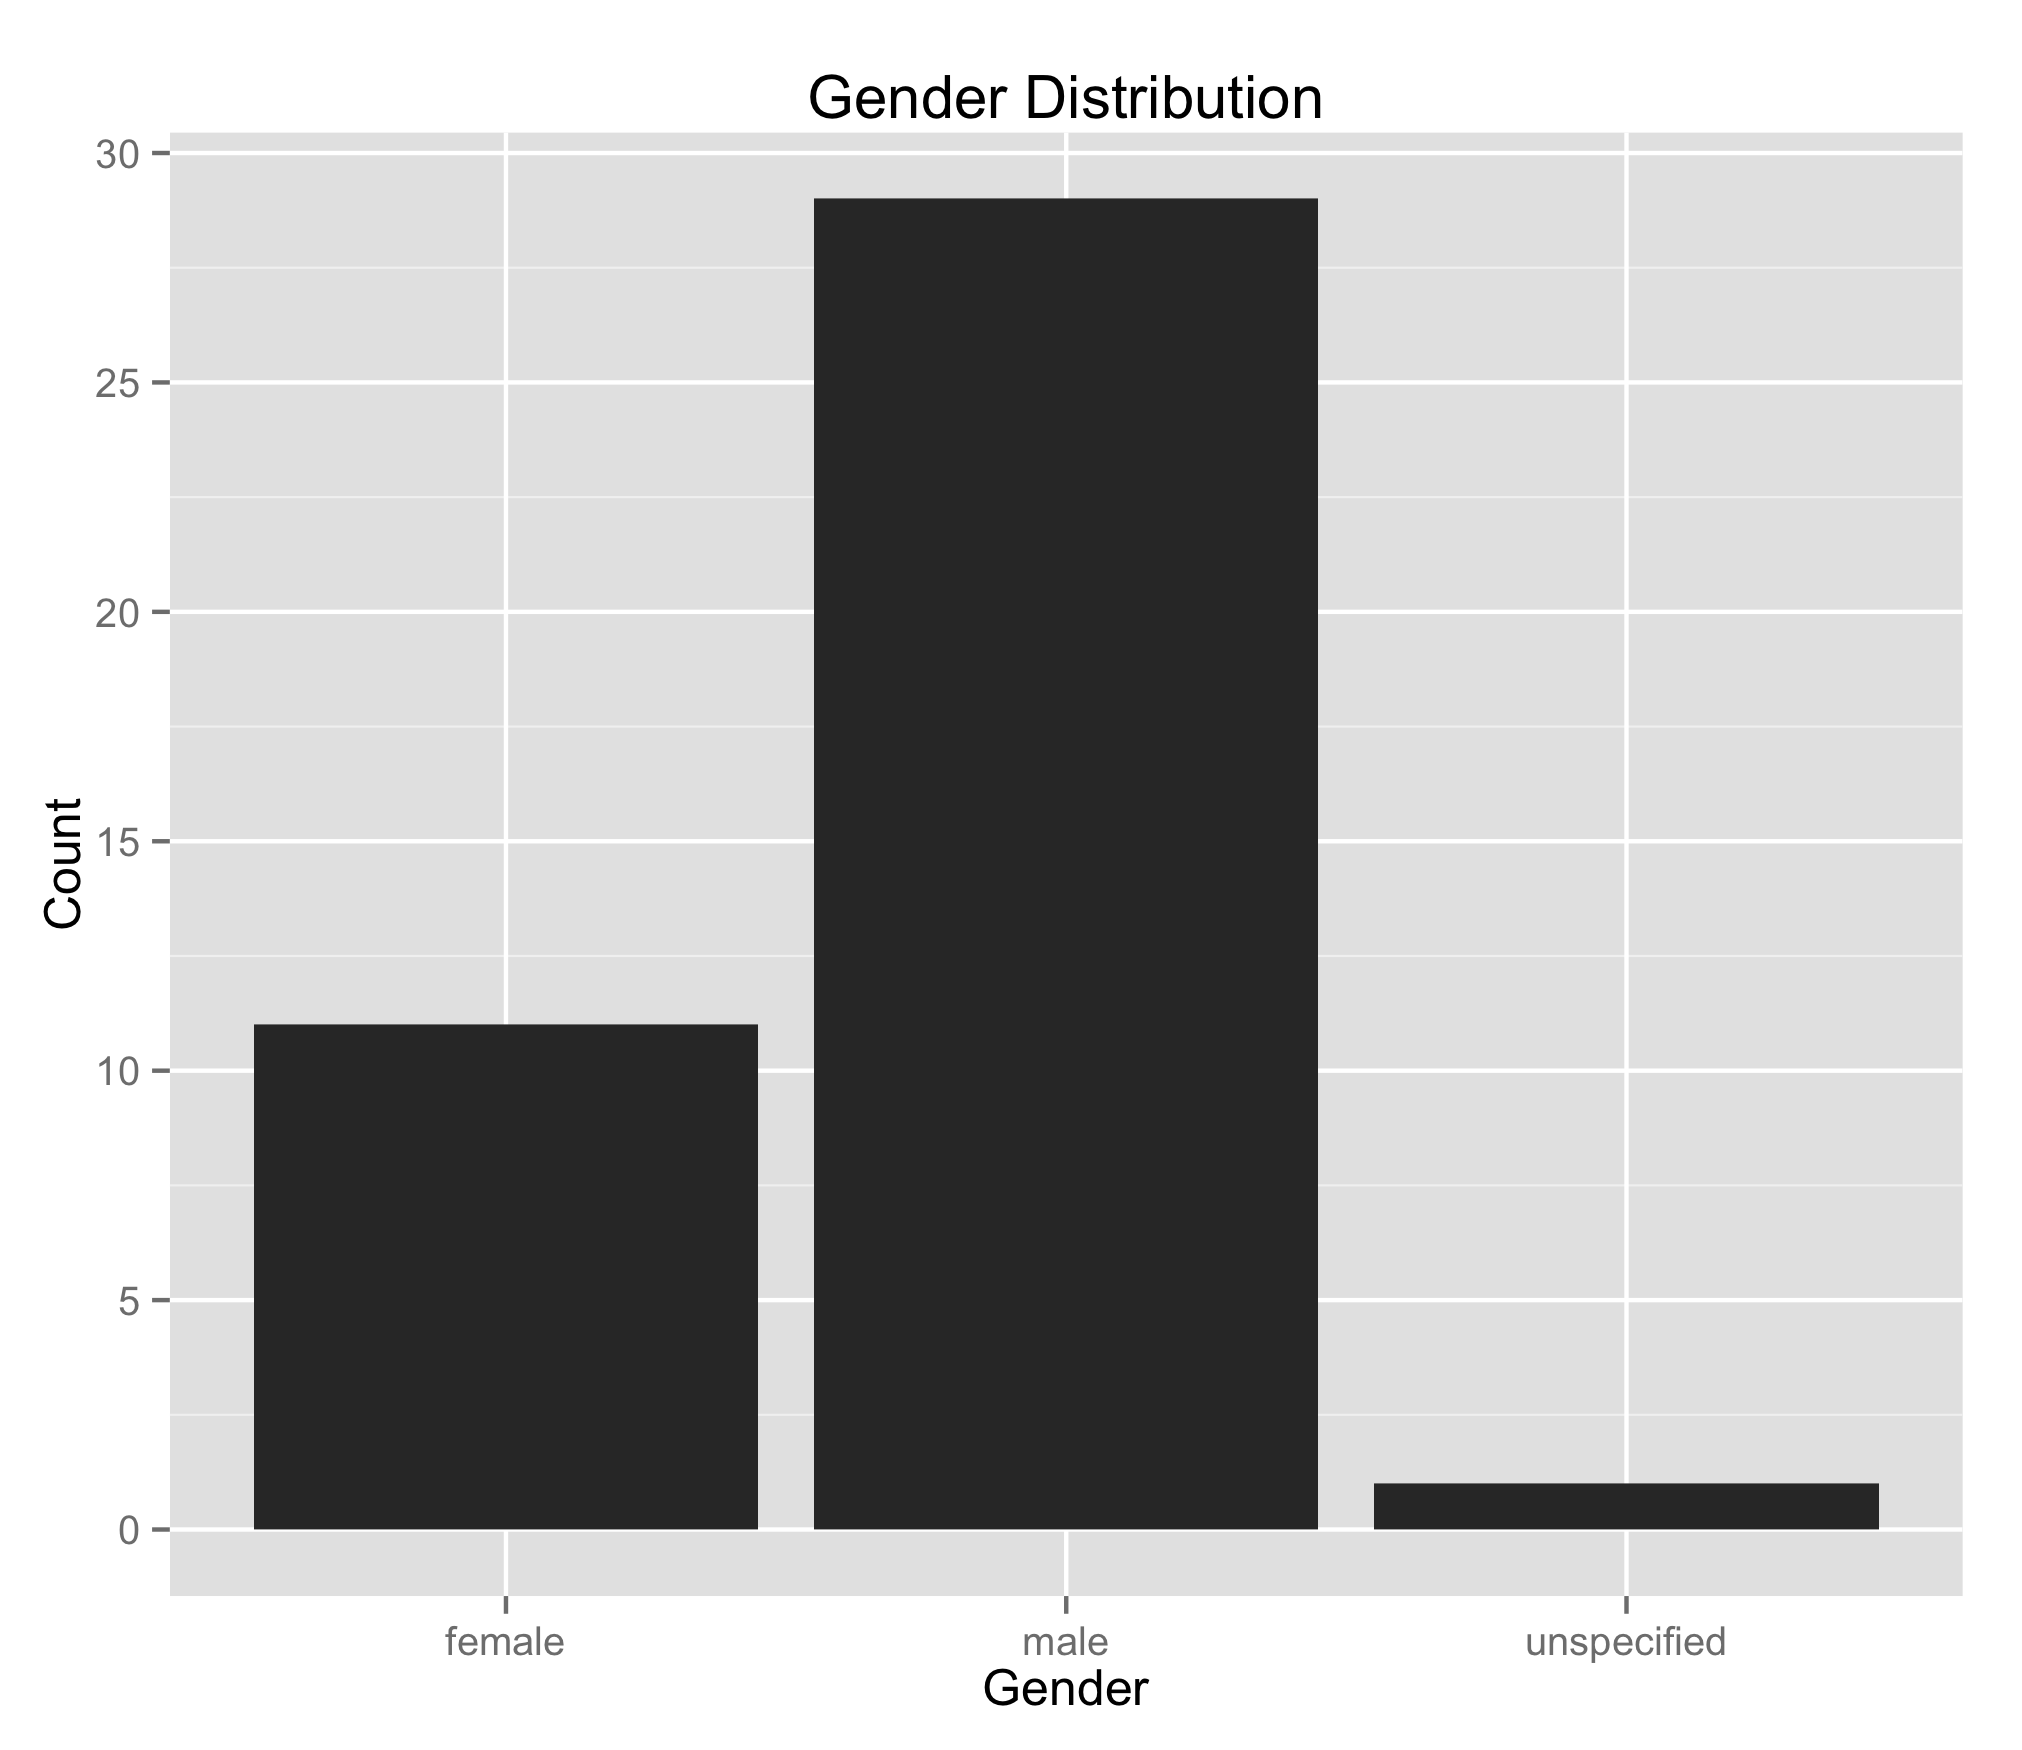
\includegraphics[width=1.0\linewidth]{gender.png}
    \caption{Gender Distribution}
    \label{genderdistribution}
\end{subfigure}
\caption{Basic Demographics}
\end{figure}


\begin{figure}[t]
\centering
\begin{subfigure}{.5\textwidth}
    \centering
    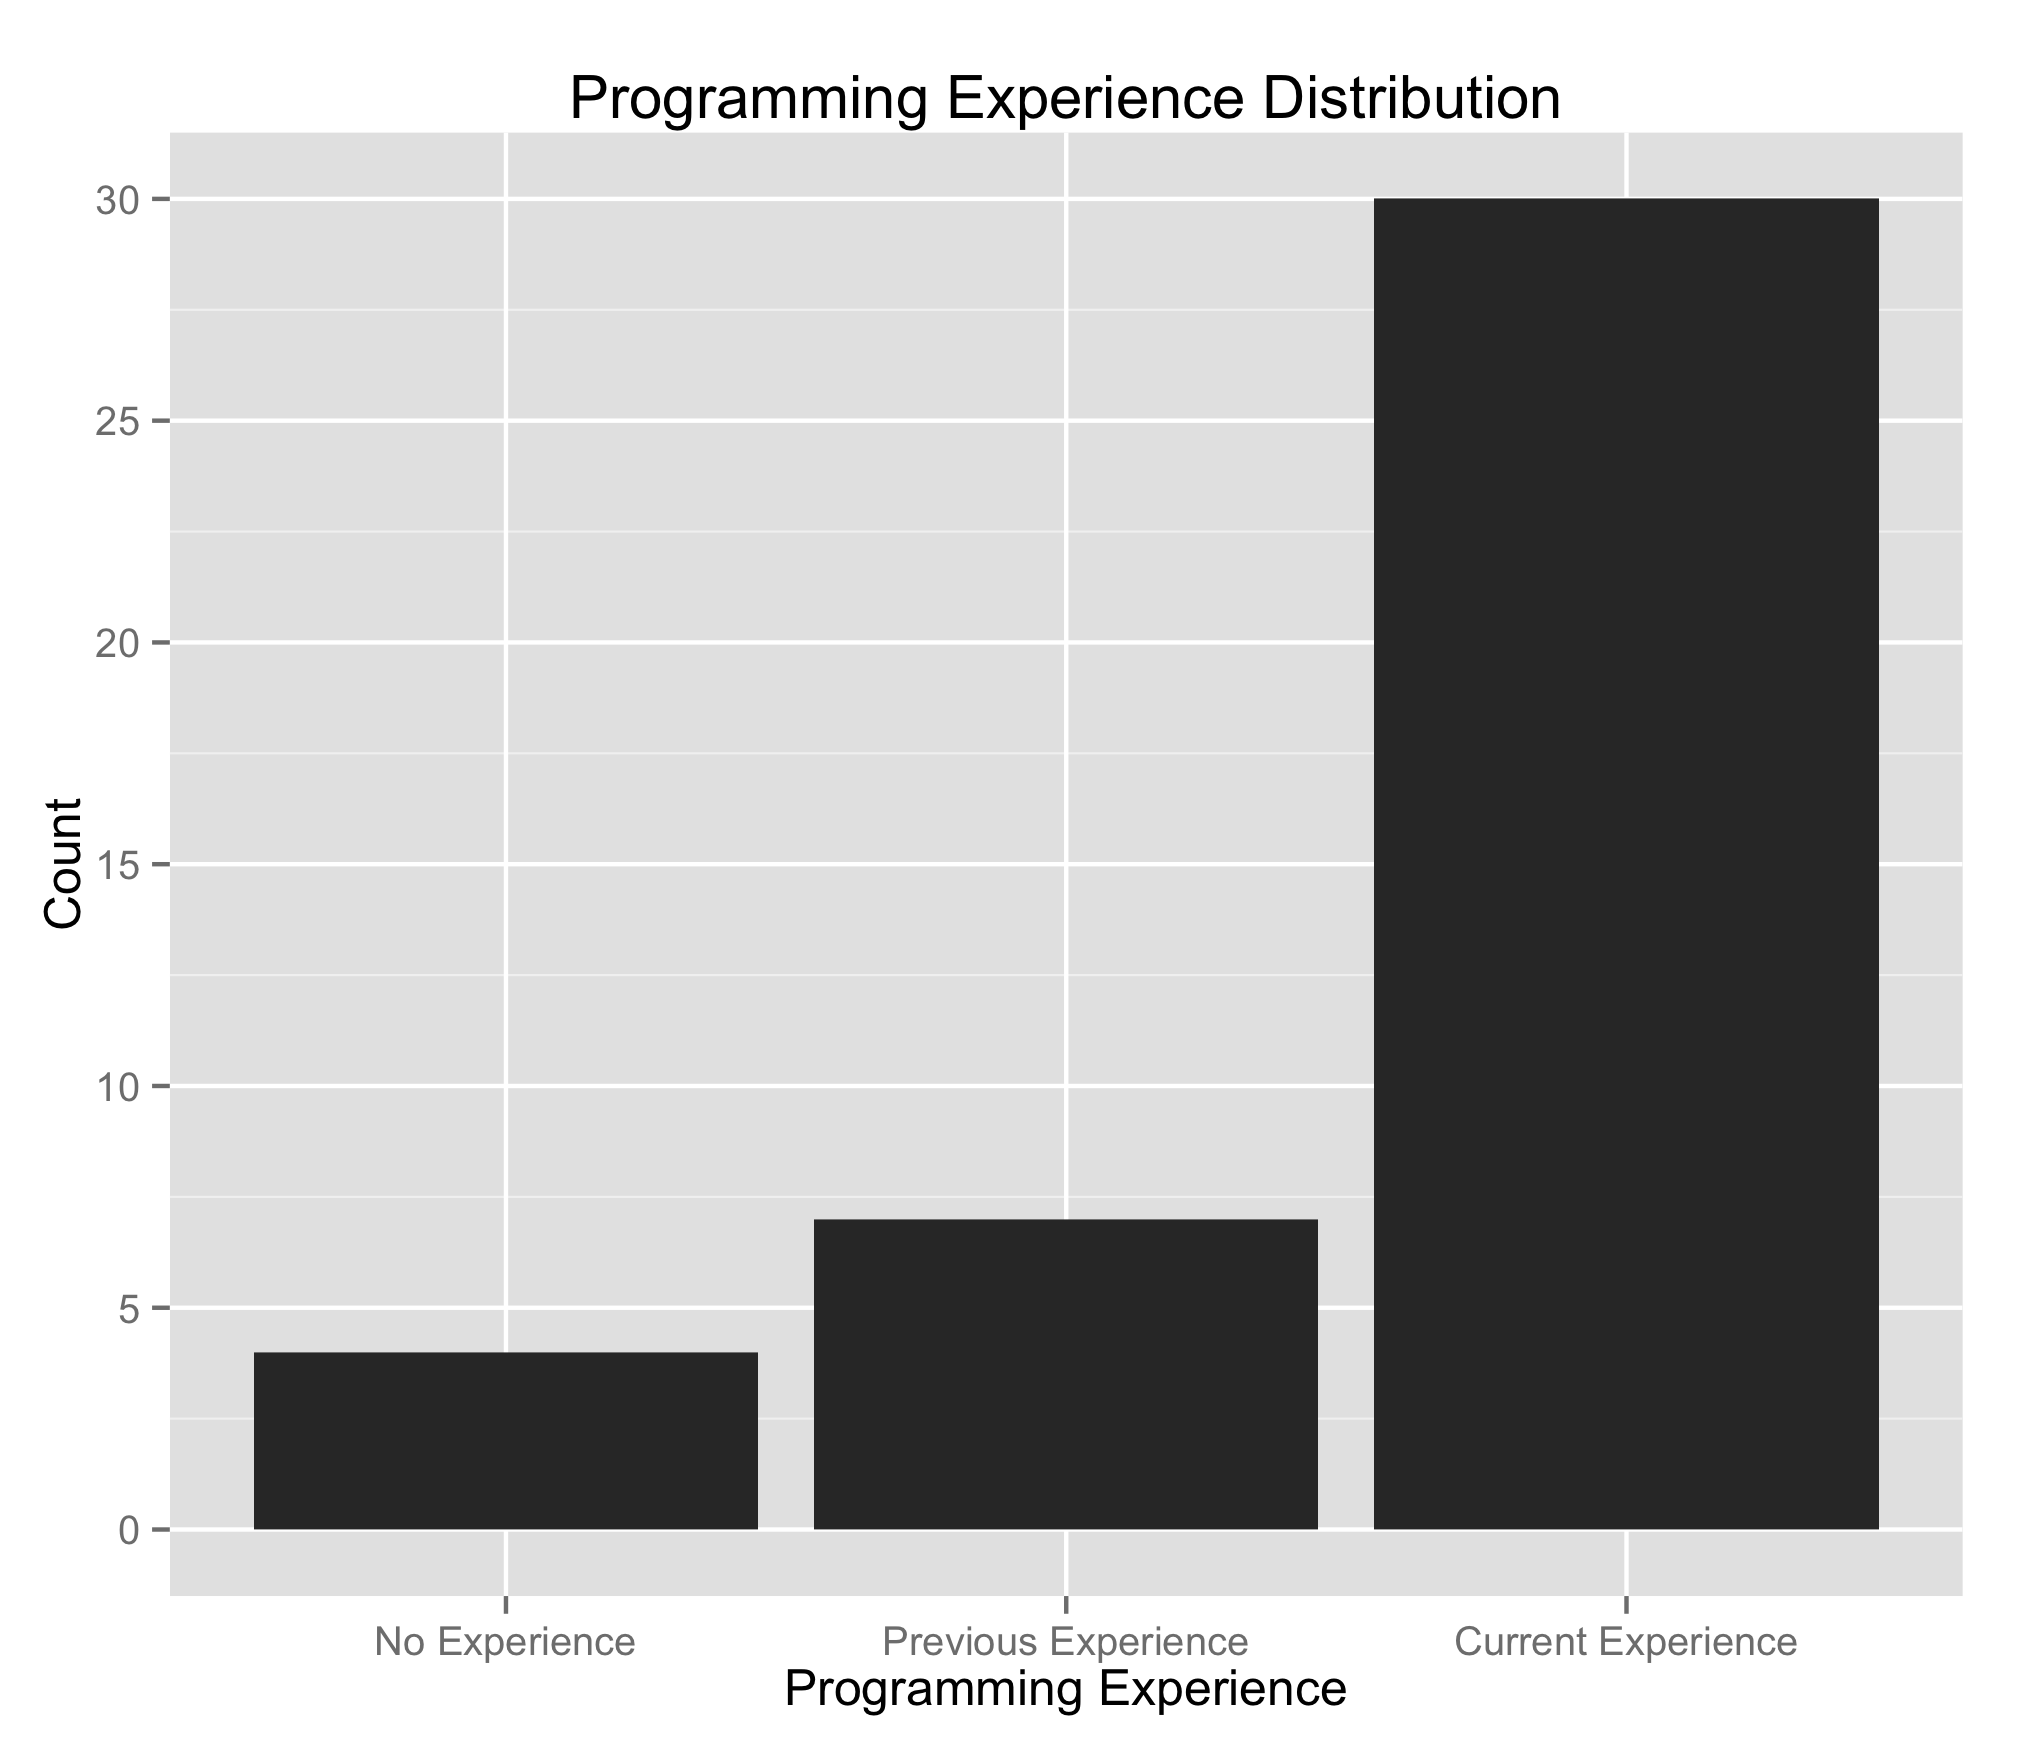
\includegraphics[width=1.0\linewidth]{programming.png}
    \caption{Programming Experience Distribution}
    \label{programmingdistribution}
\end{subfigure}%
\begin{subfigure}{.5\textwidth}
    \centering
    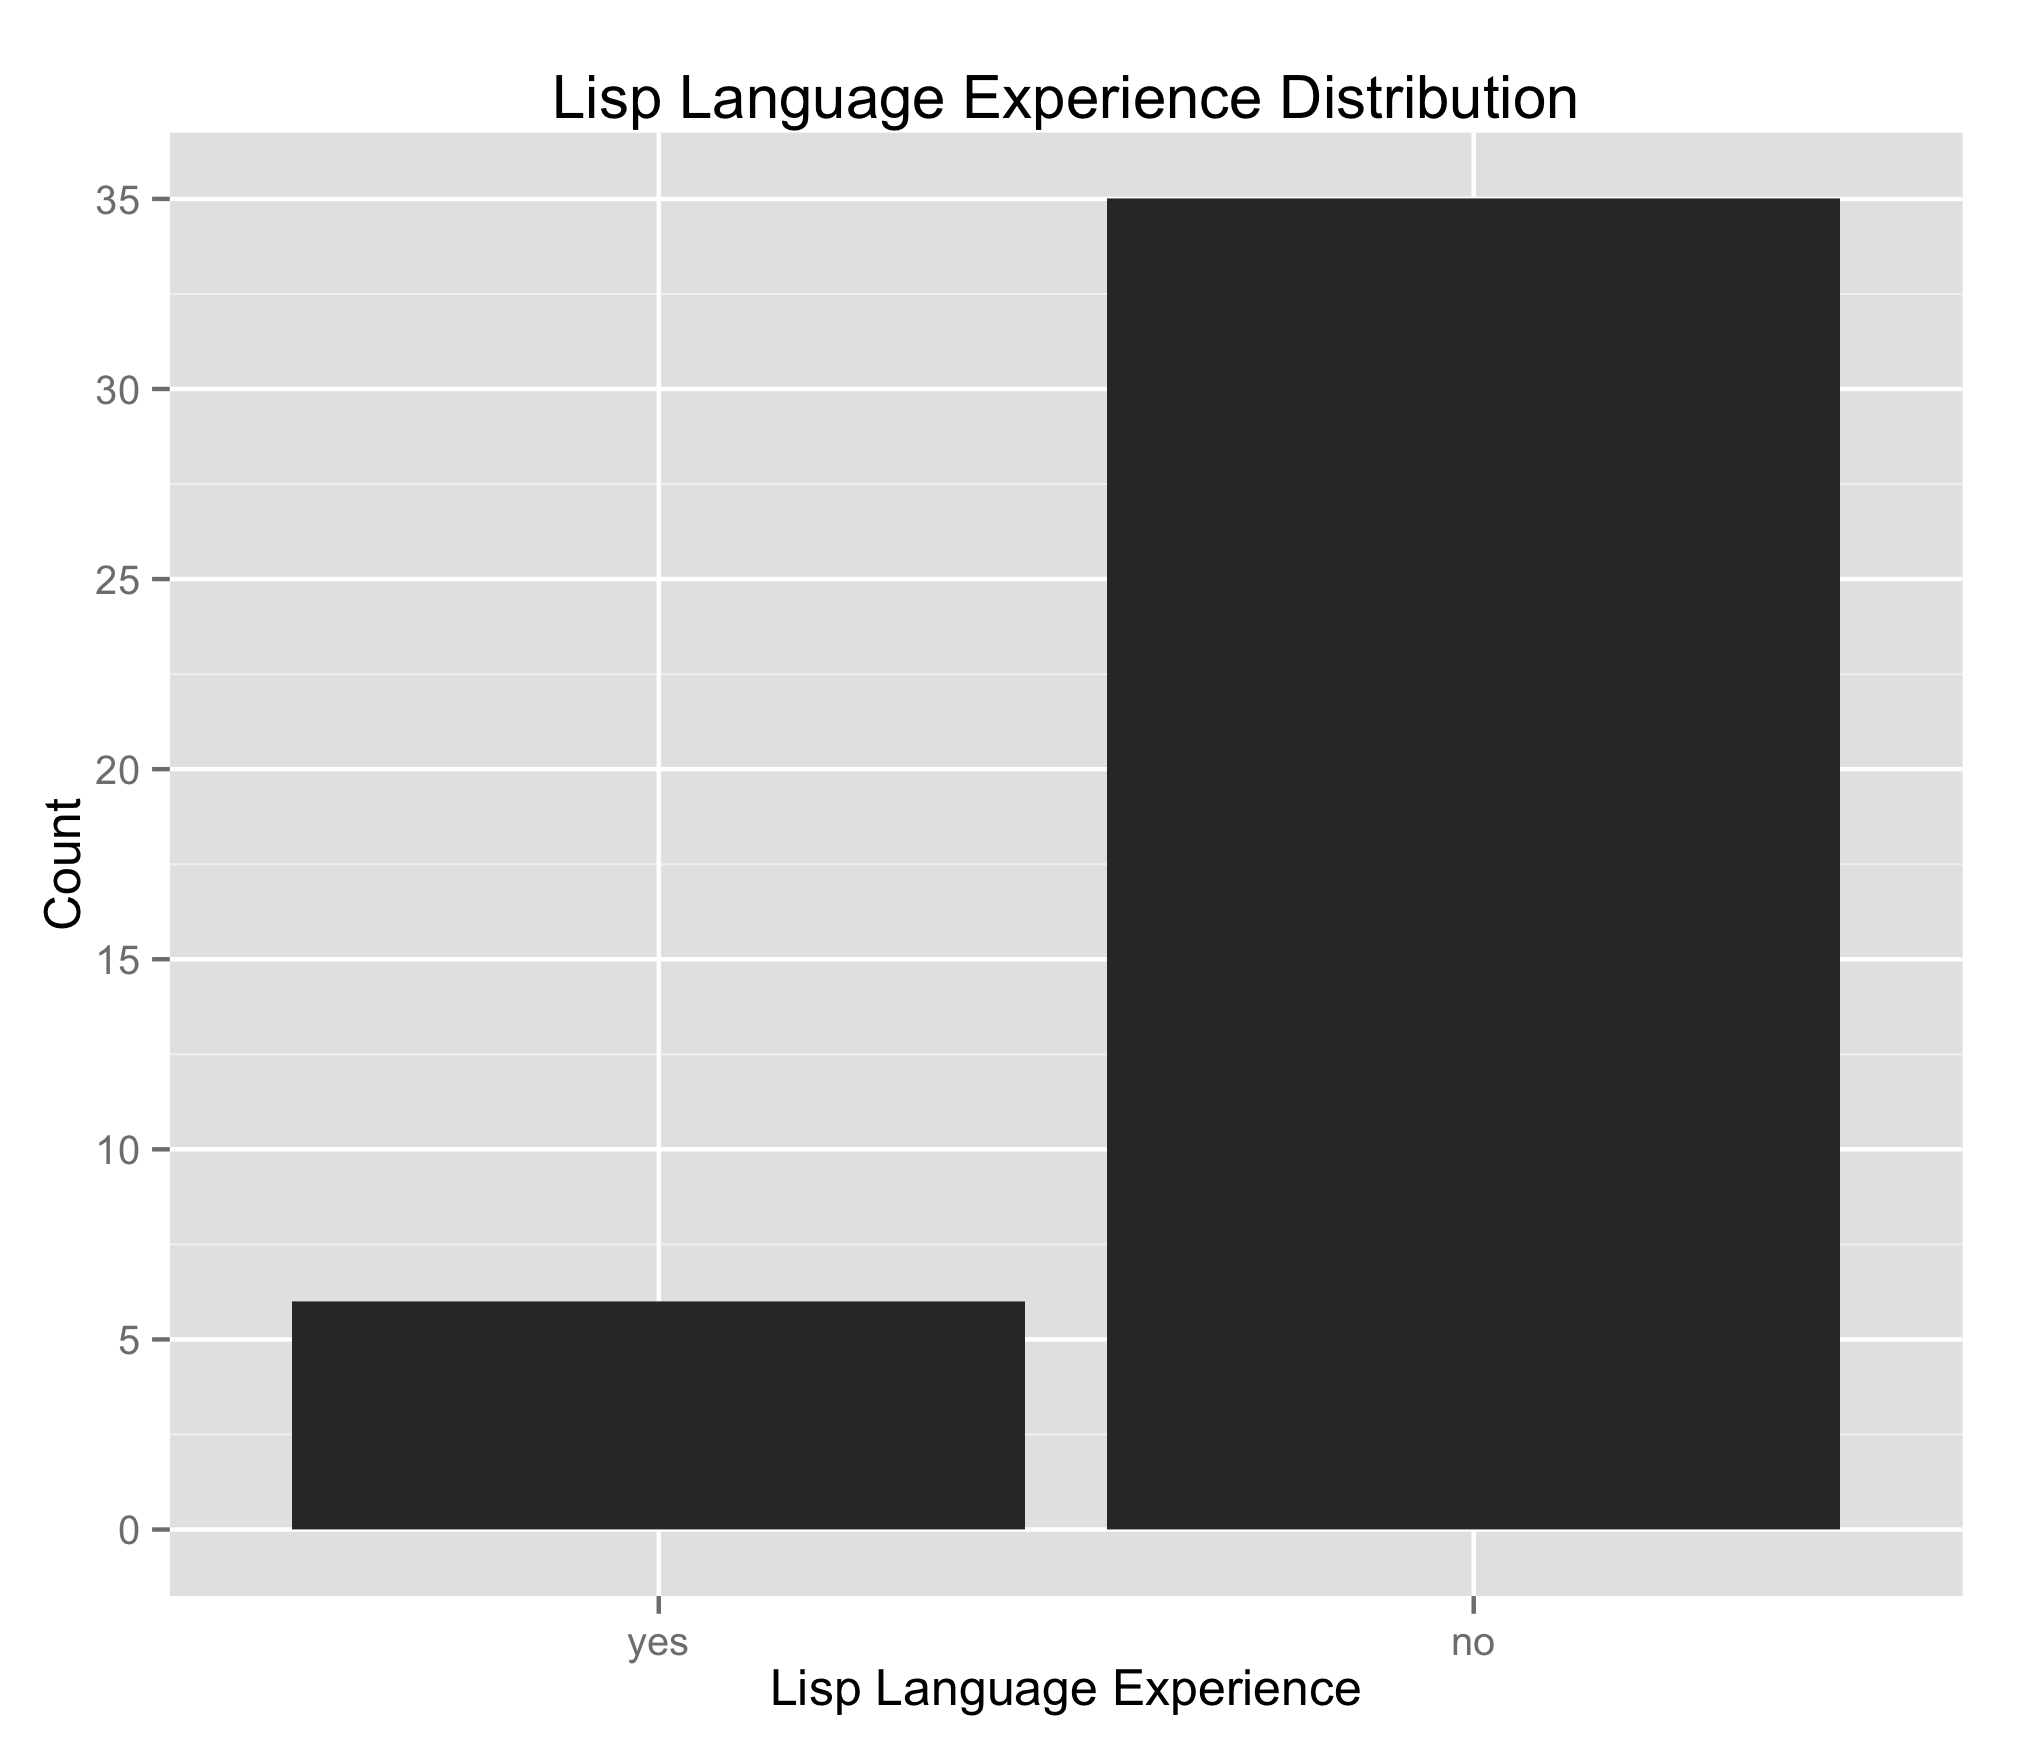
\includegraphics[width=1.0\linewidth]{lisp.png}
    \caption{Lisp Experience Distribution}
    \label{lispdistribution}
\end{subfigure}
\caption{Programming Demographics}
\end{figure}


\begin{figure}[t]
\centering
\begin{subfigure}{.5\textwidth}
    \centering
    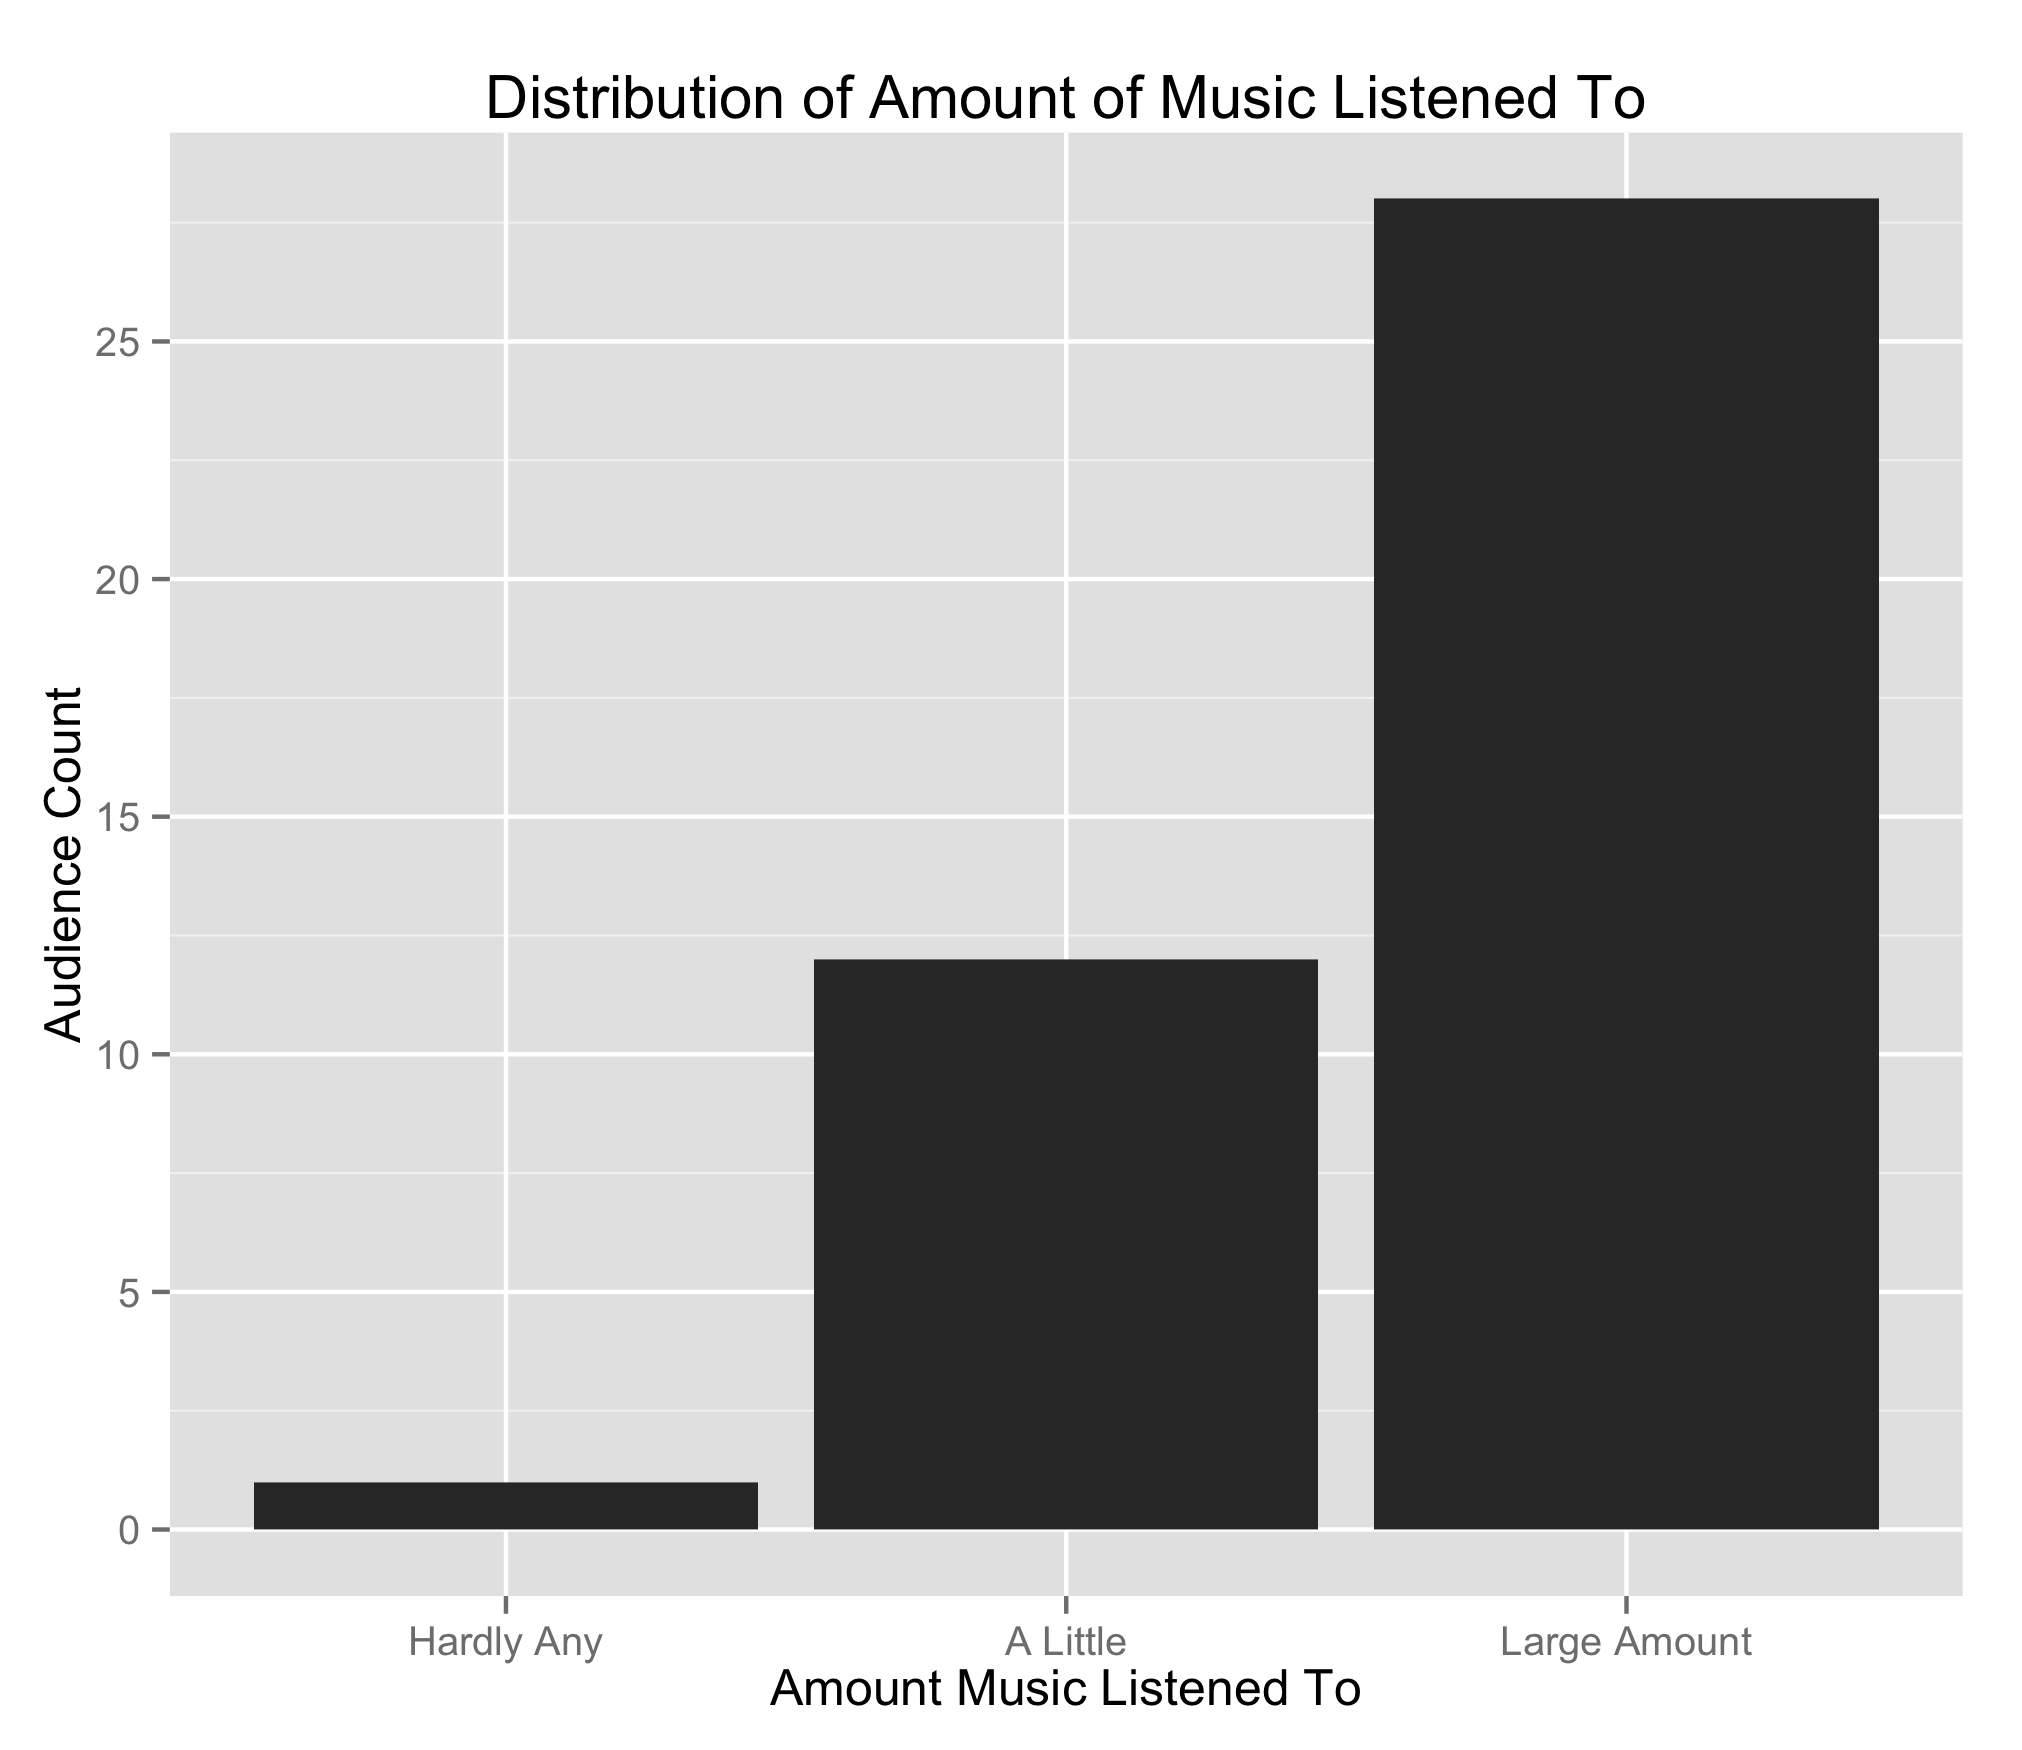
\includegraphics[width=1.0\linewidth]{music.png}
    \caption{Listen to Music Regularity Distribution}
    \label{musicdistribution}
\end{subfigure}%
\begin{subfigure}{.5\textwidth}
    \centering
    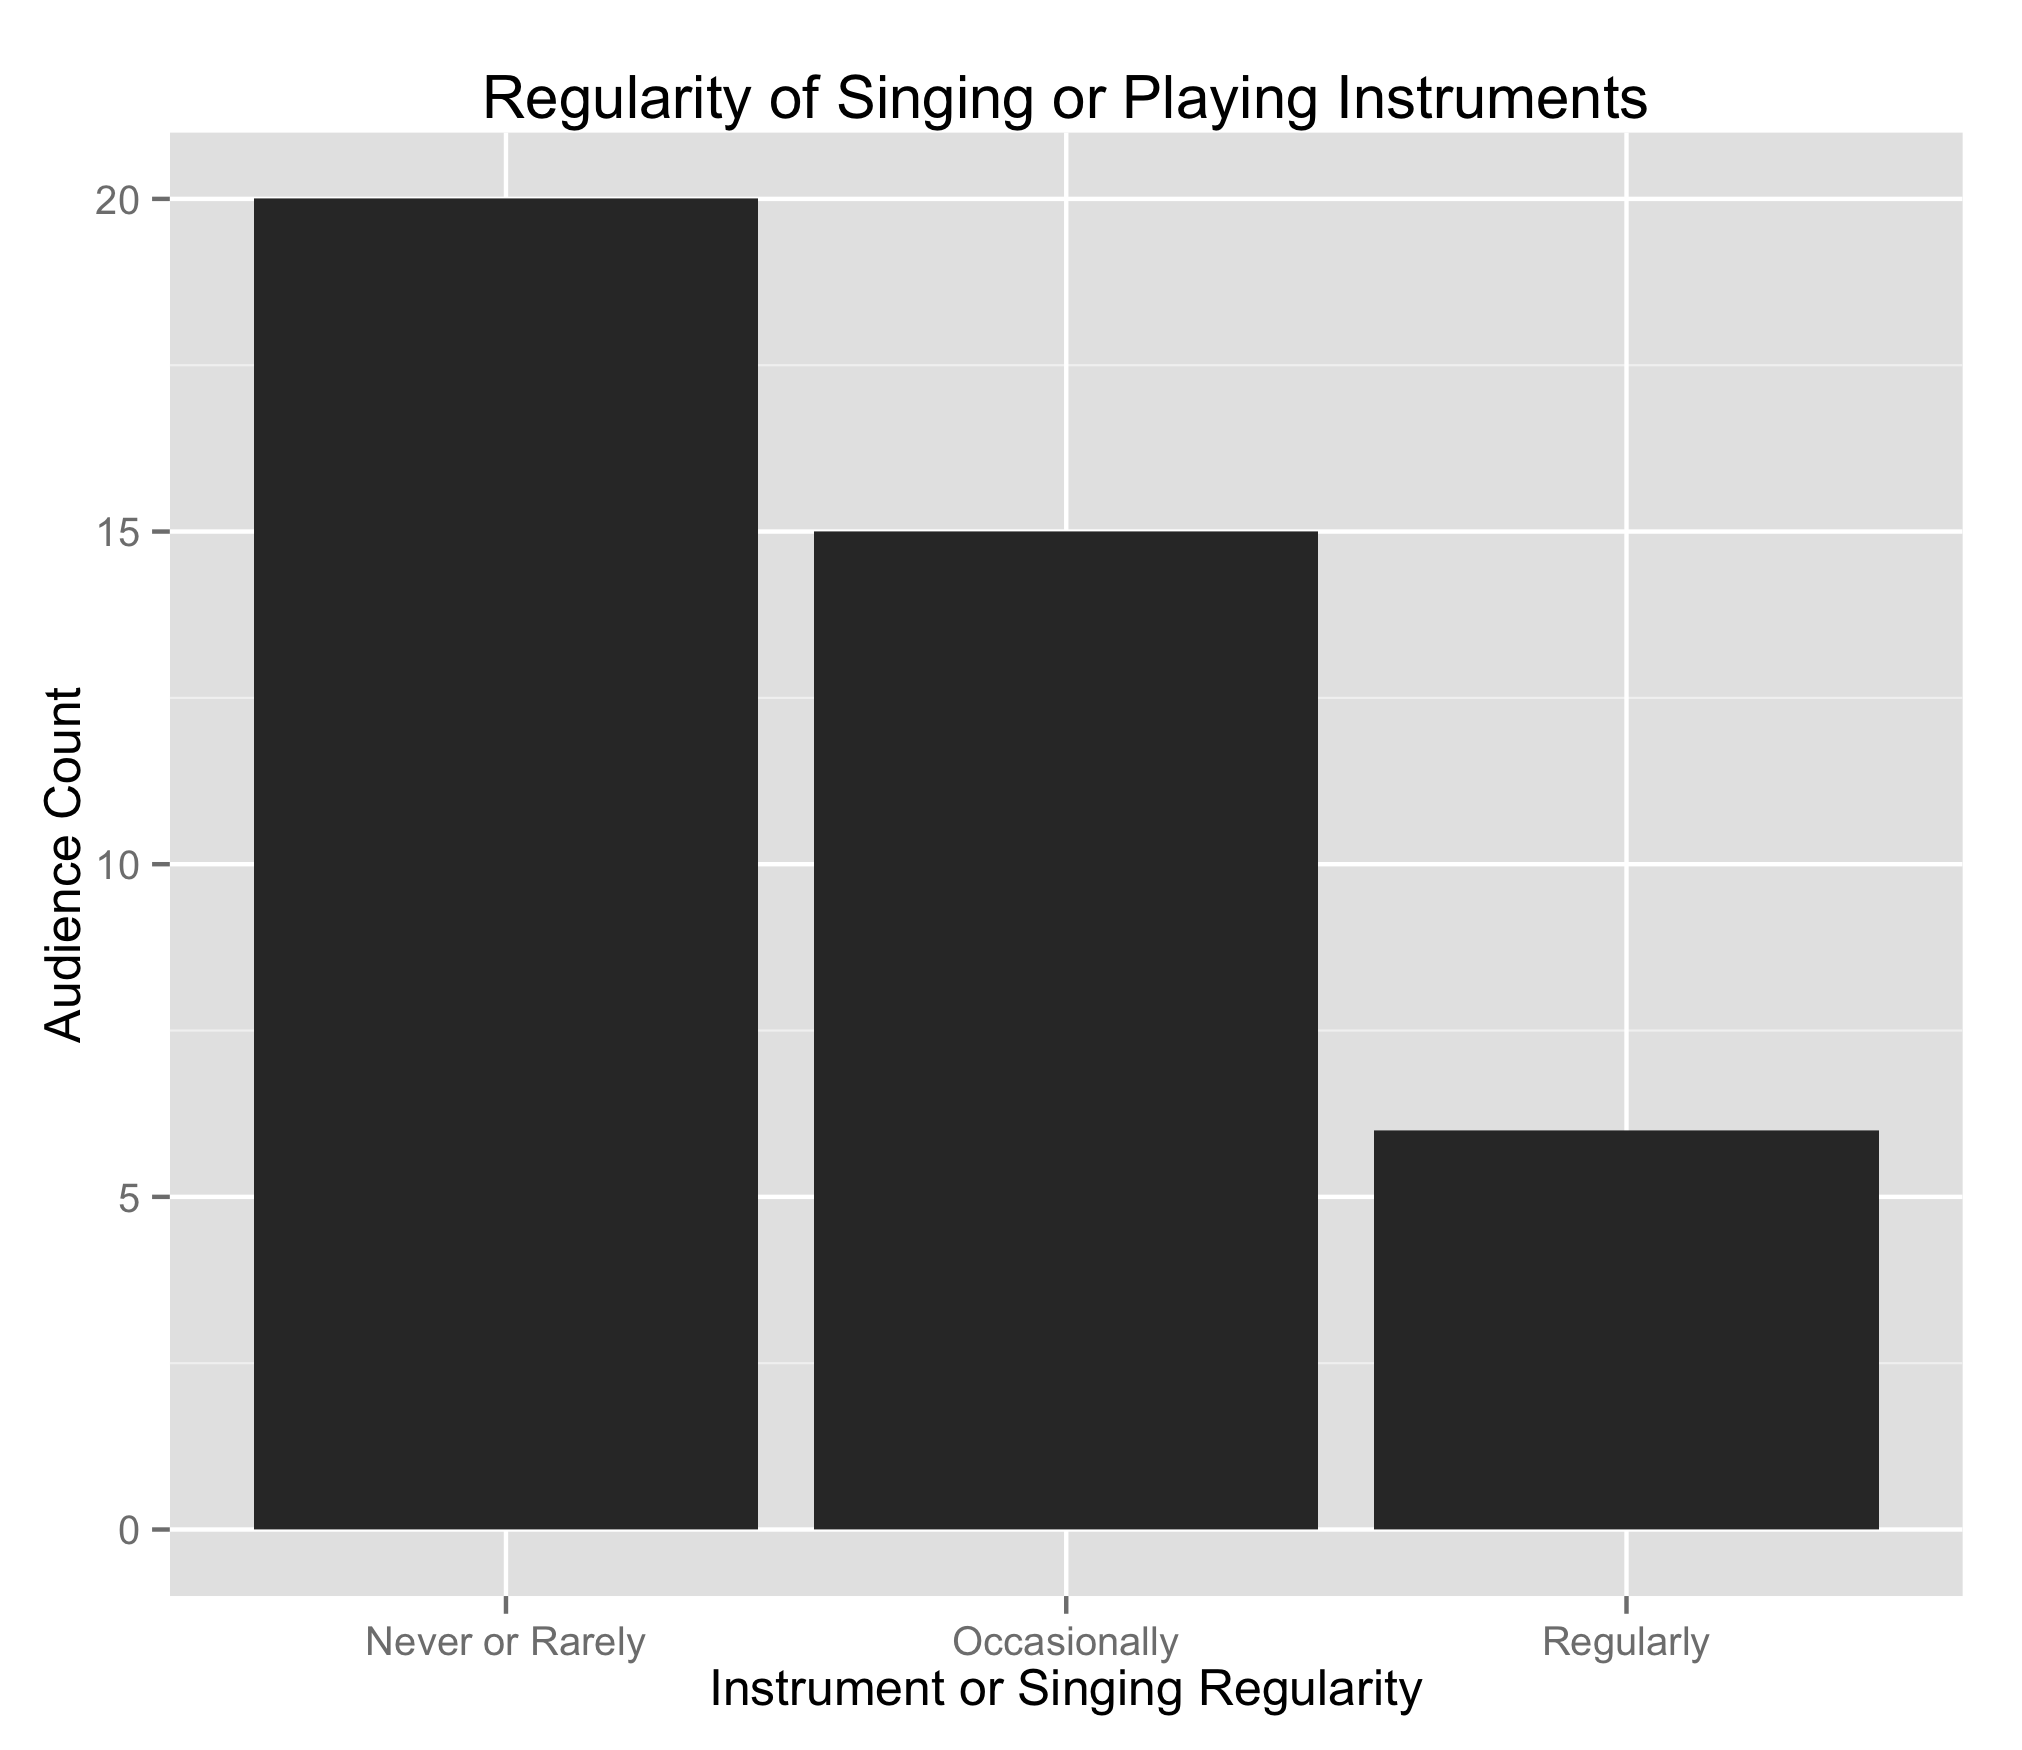
\includegraphics[width=1.0\linewidth]{instrument-regularity.png}
    \caption{Playing Instrument or Singing Regularity Distribution}
    \label{instrumentdistribution}
\end{subfigure}
\caption{Musical Demographics}
\end{figure}

\section{Results}

\subsection{Aesthetic vs Didactic Visualisation}

For the following statistical analysis a significance level of $0.05$ will be used with the chi-squared test for independence.\\

Understanding and enjoyment trends throughout the performance are available in Table \ref{tab:understandtrend} and Table \ref{tab:enjoytrend}.

\subsubsection{Understanding}
Overall, 15 participants stated specifically that the didactic visualisations helped them to understand the code, whereas 26 participants stated that the aesthetic visualisations did not assist in understanding the code. See Table \ref{tab:helpunderstand}.\\

$H_0$: There is no difference between the aesthetic visualisations and didactic visualisations in terms of understanding.\\
$H_1$: There is a difference between the two visualisations in terms of understanding.\\

Significant difference between the visualisations effect on understanding were found ($\chi^2=7.1986,df=2,p=0.02734$).


\begin{table}
\caption {Help Understanding by Participant Count} \label{tab:helpunderstand} 
\begin{center}
\begin{tabular}{ l | c c c c }

&Yes&No&No Opinion\\
\hline
Aesthetic&5&26&10 \\
Didactic&15&21&5 \\
\end{tabular}
\end{center}
\end{table}


\subsubsection{Enjoyment}
Overall, for both visualisations, a large proportion ($> 50\%$) of the participants stated that the visualisations helped their enjoyment of the performance. See Table \ref{tab:helpenjoy}.\\

$H_0$: There is no difference between the aesthetic visualisations and didactic visualisations in terms of enjoyment.\\
$H_1$: There is a difference between the two visualisations in terms of enjoyment.\\

No significant difference between the two visualisations effect on enjoyment were found ($\chi^2=3.7733,df=2,p=0.1516$).

\begin{table}
\caption {Helped Enjoyment by Participant Count} \label{tab:helpenjoy} 
\begin{center}
\begin{tabular}{ l | c c c c }

&Yes&No&No Opinion\\
\hline
Aesthetic&31&5&5 \\
Didactic&24&12&5 \\
\end{tabular}
\end{center}
\end{table}




\begin{table}
\caption {Understanding Trend by Participant Count} \label{tab:understandtrend} 
\begin{center}
\begin{tabular}{ l | c c c c }

&Up&Down&Flat&Unspecified\\
\hline
Aesthetic&13&8&18&2 \\
Didactic&15&4&20&2 \\
\end{tabular}
\end{center}
\end{table}


\begin{table}
\caption {Enjoyment Trend by Participant Count} \label{tab:enjoytrend} 
\begin{center}
\begin{tabular}{ l | c c c c }

&Up&Down&Flat&Unspecified\\
\hline
Aesthetic&15&11&13&1 \\
Didactic&15&12&14&0 \\
\end{tabular}
\end{center}
\end{table}


\section{Discussion}

In general, the visualisations contribution to enjoyment was fairly positive. This was the case for both visualisations. For understanding however, only the didactic visualisation assisted understanding during the performance.\\

A number of participants stated that the didactic visualisations were distracting, too abrupt or took away from the code in other ways. On the other hand, some said that the didactic visualisations gave the performance a sense of being 'too polished'. The general consensus, however, was that the visualisation should either better reflect the code, better reflect the music or have more variety.\\

The response to the aesthetic visualisation [...more discussion to come]

\end{document}